% Options for packages loaded elsewhere
\PassOptionsToPackage{unicode}{hyperref}
\PassOptionsToPackage{hyphens}{url}
%


\PassOptionsToPackage{table}{xcolor}

\documentclass[
  10pt,
  letterpaper,
]{article}

\usepackage{amsmath,amssymb}
\usepackage{lmodern}
\usepackage{iftex}
\ifPDFTeX
  \usepackage[T1]{fontenc}
  \usepackage[utf8]{inputenc}
  \usepackage{textcomp} % provide euro and other symbols
\else % if luatex or xetex
  \usepackage{unicode-math}
  \defaultfontfeatures{Scale=MatchLowercase}
  \defaultfontfeatures[\rmfamily]{Ligatures=TeX,Scale=1}
\fi
% Use upquote if available, for straight quotes in verbatim environments
\IfFileExists{upquote.sty}{\usepackage{upquote}}{}
\IfFileExists{microtype.sty}{% use microtype if available
  \usepackage[]{microtype}
  \UseMicrotypeSet[protrusion]{basicmath} % disable protrusion for tt fonts
}{}
\makeatletter
\@ifundefined{KOMAClassName}{% if non-KOMA class
  \IfFileExists{parskip.sty}{%
    \usepackage{parskip}
  }{% else
    \setlength{\parindent}{0pt}
    \setlength{\parskip}{6pt plus 2pt minus 1pt}}
}{% if KOMA class
  \KOMAoptions{parskip=half}}
\makeatother
\usepackage{xcolor}
\usepackage[top=0.85in,left=2.75in,footskip=0.75in]{geometry}
\setlength{\emergencystretch}{3em} % prevent overfull lines
\setcounter{secnumdepth}{-\maxdimen} % remove section numbering


\providecommand{\tightlist}{%
  \setlength{\itemsep}{0pt}\setlength{\parskip}{0pt}}\usepackage{longtable,booktabs,array}
\usepackage{calc} % for calculating minipage widths
% Correct order of tables after \paragraph or \subparagraph
\usepackage{etoolbox}
\makeatletter
\patchcmd\longtable{\par}{\if@noskipsec\mbox{}\fi\par}{}{}
\makeatother
% Allow footnotes in longtable head/foot
\IfFileExists{footnotehyper.sty}{\usepackage{footnotehyper}}{\usepackage{footnote}}
\makesavenoteenv{longtable}
\usepackage{graphicx}
\makeatletter
\def\maxwidth{\ifdim\Gin@nat@width>\linewidth\linewidth\else\Gin@nat@width\fi}
\def\maxheight{\ifdim\Gin@nat@height>\textheight\textheight\else\Gin@nat@height\fi}
\makeatother
% Scale images if necessary, so that they will not overflow the page
% margins by default, and it is still possible to overwrite the defaults
% using explicit options in \includegraphics[width, height, ...]{}
\setkeys{Gin}{width=\maxwidth,height=\maxheight,keepaspectratio}
% Set default figure placement to htbp
\makeatletter
\def\fps@figure{htbp}
\makeatother

% Use adjustwidth environment to exceed column width (see example table in text)
\usepackage{changepage}

% marvosym package for additional characters
\usepackage{marvosym}

% cite package, to clean up citations in the main text. Do not remove.
% Using natbib instead
% \usepackage{cite}

% Use nameref to cite supporting information files (see Supporting Information section for more info)
\usepackage{nameref,hyperref}

% line numbers
\usepackage[right]{lineno}

% ligatures disabled
\usepackage{microtype}
\DisableLigatures[f]{encoding = *, family = * }

% create "+" rule type for thick vertical lines
\newcolumntype{+}{!{\vrule width 2pt}}

% create \thickcline for thick horizontal lines of variable length
\newlength\savedwidth
\newcommand\thickcline[1]{%
  \noalign{\global\savedwidth\arrayrulewidth\global\arrayrulewidth 2pt}%
  \cline{#1}%
  \noalign{\vskip\arrayrulewidth}%
  \noalign{\global\arrayrulewidth\savedwidth}%
}

% \thickhline command for thick horizontal lines that span the table
\newcommand\thickhline{\noalign{\global\savedwidth\arrayrulewidth\global\arrayrulewidth 2pt}%
\hline
\noalign{\global\arrayrulewidth\savedwidth}}

% Text layout
\raggedright
\setlength{\parindent}{0.5cm}
\textwidth 5.25in 
\textheight 8.75in

% Bold the 'Figure #' in the caption and separate it from the title/caption with a period
% Captions will be left justified
\usepackage[aboveskip=1pt,labelfont=bf,labelsep=period,justification=raggedright,singlelinecheck=off]{caption}
\renewcommand{\figurename}{Fig}

% Remove brackets from numbering in List of References
\makeatletter
\renewcommand{\@biblabel}[1]{\quad#1.}
\makeatother

% Header and Footer with logo
\usepackage{lastpage,fancyhdr}
\usepackage{epstopdf}
%\pagestyle{myheadings}
\pagestyle{fancy}
\fancyhf{}
%\setlength{\headheight}{27.023pt}
%\lhead{\includegraphics[width=2.0in]{PLOS-submission.eps}}
\rfoot{\thepage/\pageref{LastPage}}
\renewcommand{\headrulewidth}{0pt}
\renewcommand{\footrule}{\hrule height 2pt \vspace{2mm}}
\fancyheadoffset[L]{2.25in}
\fancyfootoffset[L]{2.25in}
\lfoot{\today}
\makeatletter
\makeatother
\makeatletter
\makeatother
\makeatletter
\@ifpackageloaded{caption}{}{\usepackage{caption}}
\AtBeginDocument{%
\ifdefined\contentsname
  \renewcommand*\contentsname{Table of contents}
\else
  \newcommand\contentsname{Table of contents}
\fi
\ifdefined\listfigurename
  \renewcommand*\listfigurename{List of Figures}
\else
  \newcommand\listfigurename{List of Figures}
\fi
\ifdefined\listtablename
  \renewcommand*\listtablename{List of Tables}
\else
  \newcommand\listtablename{List of Tables}
\fi
\ifdefined\figurename
  \renewcommand*\figurename{Figure}
\else
  \newcommand\figurename{Figure}
\fi
\ifdefined\tablename
  \renewcommand*\tablename{Table}
\else
  \newcommand\tablename{Table}
\fi
}
\@ifpackageloaded{float}{}{\usepackage{float}}
\floatstyle{ruled}
\@ifundefined{c@chapter}{\newfloat{codelisting}{h}{lop}}{\newfloat{codelisting}{h}{lop}[chapter]}
\floatname{codelisting}{Listing}
\newcommand*\listoflistings{\listof{codelisting}{List of Listings}}
\makeatother
\makeatletter
\@ifpackageloaded{caption}{}{\usepackage{caption}}
\@ifpackageloaded{subcaption}{}{\usepackage{subcaption}}
\makeatother
\makeatletter
\makeatother
\ifLuaTeX
  \usepackage{selnolig}  % disable illegal ligatures
\fi
\usepackage[numbers,square,comma]{natbib}
\bibliographystyle{plos2015}
\IfFileExists{bookmark.sty}{\usepackage{bookmark}}{\usepackage{hyperref}}
\IfFileExists{xurl.sty}{\usepackage{xurl}}{} % add URL line breaks if available
\urlstyle{same} % disable monospaced font for URLs
\hypersetup{
  pdftitle={Working Paper},
  pdfauthor={Witek ten Hove; Ger Koole; Joost Berkhout},
  hidelinks,
  pdfcreator={LaTeX via pandoc}}



\begin{document}
\vspace*{0.2in}

% Title must be 250 characters or less.
\begin{flushleft}
{\Large
\textbf\newline{Working
Paper} % Please use "sentence case" for title and headings (capitalize only the first word in a title (or heading), the first word in a subtitle (or subheading), and any proper nouns).
}
\newline
\\
% Insert author names, affiliations and corresponding author email (do not include titles, positions, or degrees).
Witek ten Hove\textsuperscript{1,2\Yinyang}, Ger
Koole\textsuperscript{2\Yinyang}, Joost
Berkhout\textsuperscript{2\Yinyang}
\\
\bigskip
\textbf{1} Lectoraat Logistiek en Allianties, HAN University of Applied
Sciences, Arnhem, The Netherlands, \\ \textbf{2} Department of
Mathematics, VU, Amsterdam, The Netherlands, 
\bigskip

% Insert additional author notes using the symbols described below. Insert symbol callouts after author names as necessary.
% 
% Remove or comment out the author notes below if they aren't used.
%
% Primary Equal Contribution Note
\Yinyang These authors contributed equally to this work.

% Additional Equal Contribution Note
% Also use this double-dagger symbol for special authorship notes, such as senior authorship.
%\ddag These authors also contributed equally to this work.

% Current address notes
\textcurrency Current Address: Dept/Program/Center, Institution Name, City, State, Country % change symbol to "\textcurrency a" if more than one current address note
% \textcurrency b Insert second current address 
% \textcurrency c Insert third current address

% Deceased author note
\dag Deceased

% Group/Consortium Author Note
\textpilcrow Membership list can be found in the Acknowledgments
sections

% Use the asterisk to denote corresponding authorship and provide email address in note below.

\end{flushleft}

\section*{Abstract}
Lorem ipsum dolor sit amet, consectetur adipiscing elit. Curabitur eget
porta erat. Morbi consectetur est vel gravida pretium. Suspendisse ut
dui eu ante cursus gravida non sed sem. Nullam sapien tellus, commodo id
velit id, eleifend volutpat quam. Phasellus mauris velit, dapibus
finibus elementum vel, pulvinar non tellus. Nunc pellentesque pretium
diam, quis maximus dolor faucibus id. Nunc convallis sodales ante, ut
ullamcorper est egestas vitae. Nam sit amet enim ultrices, ultrices elit
pulvinar, volutpat risus.

\section*{Author summary}
Lorem ipsum dolor sit amet, consectetur adipiscing elit. Curabitur eget
porta erat. Morbi consectetur est vel gravida pretium. Suspendisse ut
dui eu ante cursus gravida non sed sem. Nullam sapien tellus, commodo id
velit id, eleifend volutpat quam. Phasellus mauris velit, dapibus
finibus elementum vel, pulvinar non tellus. Nunc pellentesque pretium
diam, quis maximus dolor faucibus id. Nunc convallis sodales ante, ut
ullamcorper est egestas vitae. Nam sit amet enim ultrices, ultrices elit
pulvinar, volutpat risus.

\linenumbers\hypertarget{introduction}{%
\section{Introduction}\label{introduction}}

\textbf{(Verbatim Ger Koole)} Many decision problems have a dynamic
nature, the consequences of our decisions become available step by step
over time, and can only be simulated or calculated as a Markov chain.
Decisions have long-term consequences, and these consequences are also
often of a stochastic nature. To ``remember'' these consequences the
``state'' of the system plays a crucial role. Decision problems can
roughly be divided in two types of problems: those where the decisions
are taken on the fly and are accounted for through a state change, and
those where decisions are taken upfront. The first category falls into
the framework of stochastic dynamic programming and is currently
immensely popular in AI under the name reinforcement learning. The
second is equally important but receives much less attention. Examples
are the scheduling of people in service centers such as health clinics
and call centers. Employees have to be scheduled well in advance, but
the consequences in terms of for example waiting times can only be
modeled through a stochastic process, for which simulation and Markov
chain analysis are the two prime solution methods.

Other examples are the design of energy systems and appointment
scheduling, but the list of possible applications is endless. Note that
many service systems have both types of decision problems: for example
long-term capacity and employee scheduling problems, and short-term task
scheduling and re-adjustments to the schedule.

The focus of the project is on the second type of problem. Simulation,
and to a lesser extend Markov chain analysis, are computationally costly
solution methods, and they have to be executed for multiple decisions.
Because the decision space is often multi-dimensional enumeration is not
possible. Local search can only find local optima and that is for a
fixed computational budget not even guaranteed.

Smarter methods are needed, a very interesting candidate is fitting a
machine learning model to a limited set of solutions and then try to
find the a (local) optimum. This has the advantage that, once trained,
it is much faster to use a ML model than simulation or Markov chain
analysis. This is known in the literature as surrogate models and
response surface methodology (to be checked), but the current
developments in machine learning open possibilities for new versions of
algorithms and new applications. A couple of things to look into:

- applications into for example appointment scheduling and shift
scheduling

- does an iterative approach help, where the test set consists of points
close to the optimum of the previous iteration? perhaps in combination
with linear regression with squares and interactions which gives a
global optimum?

- can knowledge about the problem (such as monotonicity in a parameter)
be included in a smart way in the prediction model?

\hypertarget{applications-for-and-purpose-of-outbound-appointment-systems}{%
\subsection{Applications for and purpose of outbound appointment
systems}\label{applications-for-and-purpose-of-outbound-appointment-systems}}

\citep{ahmadijavid_outpatient_2017} distinguish between three types of
decisions for designing Outpatient Appointment Systems (OASs):

\begin{itemize}
\tightlist
\item
  Strategic: long-term decisions that determine the determine the main
  structure of AOS.
\item
  Tactical: medium-term decisions on how patients groups or subgroups
  are processed.
\item
  Operational: short-term decisions related to efficient scheduling
  individual patients
\end{itemize}

\begin{longtable}[]{@{}
  >{\raggedright\arraybackslash}p{(\columnwidth - 6\tabcolsep) * \real{0.2252}}
  >{\raggedright\arraybackslash}p{(\columnwidth - 6\tabcolsep) * \real{0.1892}}
  >{\raggedright\arraybackslash}p{(\columnwidth - 6\tabcolsep) * \real{0.1261}}
  >{\raggedright\arraybackslash}p{(\columnwidth - 6\tabcolsep) * \real{0.4414}}@{}}
\toprule()
\begin{minipage}[b]{\linewidth}\raggedright
\end{minipage} & \begin{minipage}[b]{\linewidth}\raggedright
\textbf{Decision level}
\end{minipage} & \begin{minipage}[b]{\linewidth}\raggedright
\textbf{Code}
\end{minipage} & \begin{minipage}[b]{\linewidth}\raggedright
\textbf{Name (in alphabetical order)}
\end{minipage} \\
\midrule()
\endhead
\textbf{Design decisions} & Strategic & S1 & Access policy \\
& & S2 & Number of servers/resources \\
& & S3 & Policy on acceptance of walk-ins \\
& & S4 & \begin{minipage}[t]{\linewidth}\raggedright
Type of scheduling\\
\strut
\end{minipage} \\
\textbf{Planning decisions} & Tactical & T1 & Allocation of capacity to
patient groups \\
& & T2 & Appointment interval (slot) \\
& & T3 & Appointment scheduling window \\
& & T4 & Block size \\
& & T5 & Number of appointments in consultation session \\
& & T6 & Panel size \\
& & T7 & \begin{minipage}[t]{\linewidth}\raggedright
Priority of patient groups\\
\strut
\end{minipage} \\
& Operational & O1 & Allocation of patients to servers/resources \\
& & O2 & Appointment day \\
& & O3 & Appointment time \\
& & O4 & Patient acceptance/rejection \\
& & O5 & Patient selection from waiting list \\
& & O6 & Patient sequence \\
\bottomrule()
\end{longtable}

They labeled articles on OASs by decision type, solution method and
modeling approach.

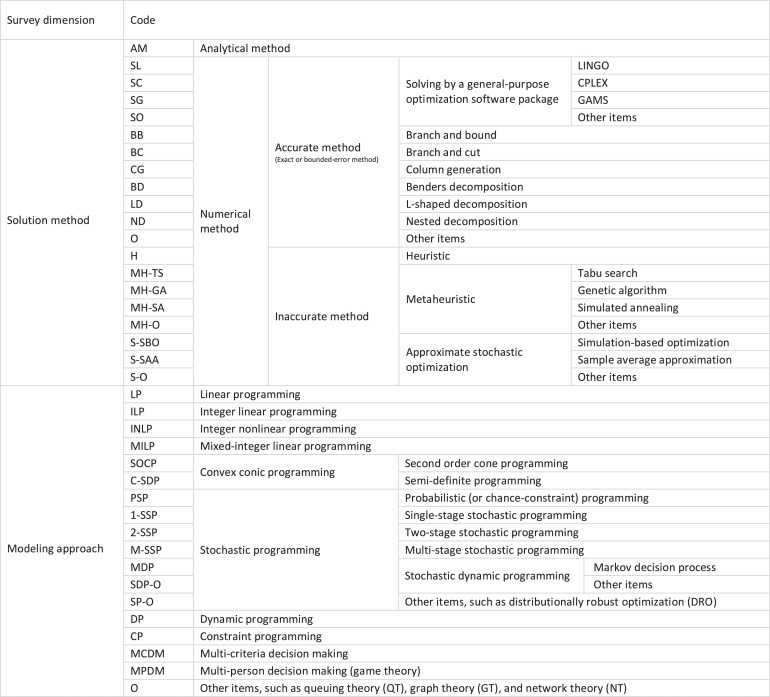
\includegraphics{images/ahmadi2.jpeg}

In this article we will be using a single-stage stochastic programming
(1-SSP) modeling approach.

\begin{longtable}[]{@{}
  >{\raggedright\arraybackslash}p{(\columnwidth - 16\tabcolsep) * \real{0.2449}}
  >{\raggedright\arraybackslash}p{(\columnwidth - 16\tabcolsep) * \real{0.1182}}
  >{\raggedright\arraybackslash}p{(\columnwidth - 16\tabcolsep) * \real{0.0445}}
  >{\raggedright\arraybackslash}p{(\columnwidth - 16\tabcolsep) * \real{0.0908}}
  >{\raggedright\arraybackslash}p{(\columnwidth - 16\tabcolsep) * \real{0.1027}}
  >{\raggedright\arraybackslash}p{(\columnwidth - 16\tabcolsep) * \real{0.1233}}
  >{\raggedright\arraybackslash}p{(\columnwidth - 16\tabcolsep) * \real{0.1849}}
  >{\raggedright\arraybackslash}p{(\columnwidth - 16\tabcolsep) * \real{0.0411}}
  >{\raggedright\arraybackslash}p{(\columnwidth - 16\tabcolsep) * \real{0.0377}}@{}}
\caption{Selection of articles taken from
\citep{ahmadijavid_outpatient_2017} with single-stage stochastic
programming (1-SSP) as the modeling approach.}\tabularnewline
\toprule()
\begin{minipage}[b]{\linewidth}\raggedright
\textbf{Reference}
\end{minipage} & \begin{minipage}[b]{\linewidth}\raggedright
\textbf{Tactical and operational decisions}
\end{minipage} & \begin{minipage}[b]{\linewidth}\raggedright
\textbf{Access policy}
\end{minipage} & \begin{minipage}[b]{\linewidth}\raggedright
\textbf{Type of scheduling: online (On), offline (Off)}
\end{minipage} & \begin{minipage}[b]{\linewidth}\raggedright
\textbf{Number of servers/resources: single (S), multiple (M)}
\end{minipage} & \begin{minipage}[b]{\linewidth}\raggedright
\textbf{Policy on acceptance of walk-ins: allowed (Yes), not allowed
(No)}
\end{minipage} & \begin{minipage}[b]{\linewidth}\raggedright
\textbf{Objective: minimize (Min.), maximize (Max.)}
\end{minipage} & \begin{minipage}[b]{\linewidth}\raggedright
\textbf{Modeling approach}
\end{minipage} & \begin{minipage}[b]{\linewidth}\raggedright
\textbf{Solution method}
\end{minipage} \\
\midrule()
\endfirsthead
\toprule()
\begin{minipage}[b]{\linewidth}\raggedright
\textbf{Reference}
\end{minipage} & \begin{minipage}[b]{\linewidth}\raggedright
\textbf{Tactical and operational decisions}
\end{minipage} & \begin{minipage}[b]{\linewidth}\raggedright
\textbf{Access policy}
\end{minipage} & \begin{minipage}[b]{\linewidth}\raggedright
\textbf{Type of scheduling: online (On), offline (Off)}
\end{minipage} & \begin{minipage}[b]{\linewidth}\raggedright
\textbf{Number of servers/resources: single (S), multiple (M)}
\end{minipage} & \begin{minipage}[b]{\linewidth}\raggedright
\textbf{Policy on acceptance of walk-ins: allowed (Yes), not allowed
(No)}
\end{minipage} & \begin{minipage}[b]{\linewidth}\raggedright
\textbf{Objective: minimize (Min.), maximize (Max.)}
\end{minipage} & \begin{minipage}[b]{\linewidth}\raggedright
\textbf{Modeling approach}
\end{minipage} & \begin{minipage}[b]{\linewidth}\raggedright
\textbf{Solution method}
\end{minipage} \\
\midrule()
\endhead
\href{https://www.sciencedirect.com/science/article/pii/S0377221716305239?via\%3Dihub\#bib0008}{\textbf{(}Begen
\& Queyranne, 2011}\textbf{)} & O3 (OBA) & Traditional & Off & S & Yes
(urgent) & Min. costs of waiting time, idle time, and overtime & 1-SSP &
AM \\
\href{https://www.sciencedirect.com/science/article/pii/S0377221716305239?via\%3Dihub\#bib0018}{\textbf{(}Chakraborty
et al., 2010}\textbf{)} & O3/O4 (OBA) (integrated) & Open-access & On &
S & No & Max. profit (revenue of patients seen -- costs of patients
overflowing between each two successive slots) & 1-SSP & AM/H \\
\href{https://www.sciencedirect.com/science/article/pii/S0377221716305239?via\%3Dihub\#bib0019}{\textbf{(}Chakraborty
et al., 2013}\textbf{)} & O3/O4 (OBA) (integrated) & Hybrid & On & S &
No & Max. profit (revenue of patients seen -- costs of waiting time and
overtime) & 1-SSP & AM/H \\
\href{https://www.sciencedirect.com/science/article/pii/S0377221716305239?via\%3Dihub\#bib0074}{\textbf{(}LaGanga
\& Lawrence, 2012}\textbf{)} & T4/T5 (integrated) & Traditional & - & S
& No & Max. profit (revenue of patients seen -- costs of waiting time
and overtime) & 1-SSP & AM/H \\
\href{https://www.sciencedirect.com/science/article/pii/S0377221716305239?via\%3Dihub\#bib0093}{\textbf{(}Muthuraman
\& Lawley, 2008}\textbf{)} & O3 (OBA) & Open-access & On & S & No & Max.
profit (revenue of patients seen -- costs of waiting time and overtime)
& 1-SSP & AM/H \\
\href{https://www.sciencedirect.com/science/article/pii/S0377221716305239?via\%3Dihub\#bib0121}{\textbf{(}Samorani
\& Ganguly, 2016}\textbf{)} & O6 (for unpunctual patient) (OBA) & - & -
& S & No & Min. costs of waiting time and idle time & 1-SSP & AM/H \\
\href{https://www.sciencedirect.com/science/article/pii/S0377221716305239?via\%3Dihub\#bib0148}{\textbf{(}Zacharias
\& Pinedo, 2014}\textbf{)} & \begin{minipage}[t]{\linewidth}\raggedright
T4/O3/O6 (heterogeneous patients) (RBA)\\
(integrated)T4/O3 (homogeneous patients) (OBA)(integrated)\strut
\end{minipage} & Traditional &
\begin{minipage}[t]{\linewidth}\raggedright
Off\\
\strut \\
\strut \\
On\strut
\end{minipage} & S & No & Min. costs of waiting time, idle time, and
overtime & 1-SSP & AM/H \\
\href{https://www.sciencedirect.com/science/article/pii/S0377221716305239?via\%3Dihub\#bib0149}{\textbf{(}Zeng
et al., 2010}\textbf{)} & \begin{minipage}[t]{\linewidth}\raggedright
T1/T4/O3 (OBA) (integrated)\\
O3/O4 (OBA) (integrated)\strut
\end{minipage} & Traditional Open-access & Off On & S & No & Max. profit
(revenue of patients seen -- costs of waiting time and overtime) & 1-SSP
- & AM/H H \\
\href{https://www.sciencedirect.com/science/article/pii/S0377221716305239?via\%3Dihub\#bib0059}{\textbf{(}Kaandorp
\& Koole, 2007}\textbf{)} & T4/O3 (OBA) (integrated) & Traditional & - &
S & No & Min. costs of waiting time, idle time, and overtime & 1-SSP &
AM/O \\
\href{https://www.sciencedirect.com/science/article/pii/S0377221716305239?via\%3Dihub\#bib0067}{\textbf{(}Koeleman
\& Koole, 2012}\textbf{)} & T4/O3 (OBA) (integrated) & - & - & S & Yes
(Urgent) & Min. costs of waiting time, idle time, and overtime & 1-SSP &
AM/O \\
\href{https://www.sciencedirect.com/science/article/pii/S0377221716305239?via\%3Dihub\#bib0151}{\textbf{(}Kong
et al., 2016}\textbf{)} & O6 & - & Off & S & No & Min. costs of waiting
time and overtime & 1-SSP & AM/O \\
\href{https://www.sciencedirect.com/science/article/pii/S0377221716305239?via\%3Dihub\#bib0113}{\textbf{(}Qu
et al., 2007}\textbf{)} & T1 & Hybrid & - & S & No & Max. \# of patients
seen & 1-SSP & AM/O \\
\href{https://www.sciencedirect.com/science/article/pii/S0377221716305239?via\%3Dihub\#bib0146}{\textbf{(}Yan
et al., 2015}\textbf{)} & O3/O4 (OBA) (integrated) & Traditional & On &
S & No & Max. profit (revenue of patients seen -- costs of waiting time,
overtime, and idle time) & 1-SSP & AM/O \\
\href{https://www.sciencedirect.com/science/article/pii/S0377221716305239?via\%3Dihub\#bib0007}{\textbf{(}Begen
et al., 2012}\textbf{)} & O3 (OBA) & Traditional & Off & S & No & Min.
costs of waiting time, idle time, and overtime & 1-SSP & AM/S-SAA \\
\href{https://www.sciencedirect.com/science/article/pii/S0377221716305239?via\%3Dihub\#bib0082}{\textbf{(}Luo
et al., 2012}\textbf{)} & T2/T5/O3 (OBA) (integrated) & Traditional & -
& S & Yes (urgent) & Max. profit (revenue of patients seen -- costs of
waiting time and overtime) & 1-SSP & AM/SO \\
\href{https://www.sciencedirect.com/science/article/pii/S0377221716305239?via\%3Dihub\#bib0021}{\textbf{(}Chen
\& Robinson, 2014}\textbf{)} &
\begin{minipage}[t]{\linewidth}\raggedright
T2/O3/O6 (T2/O3: OBA, O6: RBA)\\
(T2/O3: integrated, (T2/O3)/O6: sequential)\strut
\end{minipage} & Hybrid & On & S & No & Min. costs of waiting time, idle
time, and overtime & 1-SSP & BD/H (for O6) \\
\href{https://www.sciencedirect.com/science/article/pii/S0377221716305239?via\%3Dihub\#bib0137}{\textbf{(}Vink
et al., 2015}\textbf{)} & T2/O3 (OBA) (integrated) & Traditional & Off &
S & No & Min. costs of waiting time, idle time, and overtime & 1-SSP &
H \\
\href{https://www.sciencedirect.com/science/article/pii/S0377221716305239?via\%3Dihub\#bib0053}{\textbf{(}Hassin
\& Mendel, 2008}\textbf{)} & T2/O3 (OBA) (integrated) & Traditional &
Off & S & No & Min. costs of waiting time and server availability &
1-SSP & O \\
\href{https://www.sciencedirect.com/science/article/pii/S0377221716305239?via\%3Dihub\#bib0061}{\textbf{(}Kim
\& Giachetti, 2006}\textbf{)} & T5 & Traditional & - & S & Yes (regular)
& Max. profit (revenue of patients seen -- costs of overtime and patient
rejection) & 1-SSP & O \\
\href{https://www.sciencedirect.com/science/article/pii/S0377221716305239?via\%3Dihub\#bib0002}{\textbf{(}Anderson,
Zheng, Yoon, \& Khasawneh, 2015}\textbf{)} & T2 & Traditional & - & S &
No & Min. costs of waiting time, idle time, and overtime & 1-SSP &
S-SBO \\
\href{https://www.sciencedirect.com/science/article/pii/S0377221716305239?via\%3Dihub\#bib0015}{\textbf{(}Cayirli
\& Gunes, 2013}\textbf{)} & T1/T4 (integrated) & Hybrid & On & S & Yes
(regular) & Min. costs of waiting time, idle time, and overtime & 1-SSP
& S-SBO \\
\href{https://www.sciencedirect.com/science/article/pii/S0377221716305239?via\%3Dihub\#bib0055}{\textbf{(}Huang
\& Zuniga, 2012}\textbf{)} & T4/O3 (based on no-show threshold for each
slot) (OBA)(integrated) & - & On & S & No & Min. costs of waiting time,
idle time, and overtime & 1-SSP & S-SBO \\
\href{https://www.sciencedirect.com/science/article/pii/S0377221716305239?via\%3Dihub\#bib0054}{\textbf{(}Huang,
Hancock, \& Herrin, 2012}\textbf{)} & T2 & - & - & S & No & Min. waiting
time and idle time & 1-SSP & S-SBO \\
\href{https://www.sciencedirect.com/science/article/pii/S0377221716305239?via\%3Dihub\#bib0063}{\textbf{(}Klassen
\& Yoogalingam, 2009}\textbf{)} & T2/O3 (OBA) (integrated) & Traditional
& - & S & No & Min. costs of waiting time, idle time, and overtime &
1-SSP & S-SBO \\
\href{https://www.sciencedirect.com/science/article/pii/S0377221716305239?via\%3Dihub\#bib0064}{\textbf{(}Klassen
\& Yoogalingam, 2013}\textbf{)} & T2/O3 (OBA) (integrated) & Traditional
& - & S & No & Min. costs of waiting time and idle time & 1-SSP &
S-SBO \\
\href{https://www.sciencedirect.com/science/article/pii/S0377221716305239?via\%3Dihub\#bib0065}{\textbf{(}Klassen
\& Yoogalingam, 2014}\textbf{)} & T2/O3 (OBA) (integrated) & Traditional
& On & S & No & Min. costs of waiting time and idle time & 1-SSP &
S-SBO \\
\href{https://www.sciencedirect.com/science/article/pii/S0377221716305239?via\%3Dihub\#bib0103}{\textbf{(}Peng,
Qu, \& Shi, 2014}\textbf{)} & T1/T4/O3 (OBA) (integrated) & Hybrid & On
& S & Yes (regular) & Min. costs of waiting time, idle time, and
overtime & 1-SSP & S-SBO/MH-GA \\
\bottomrule()
\end{longtable}

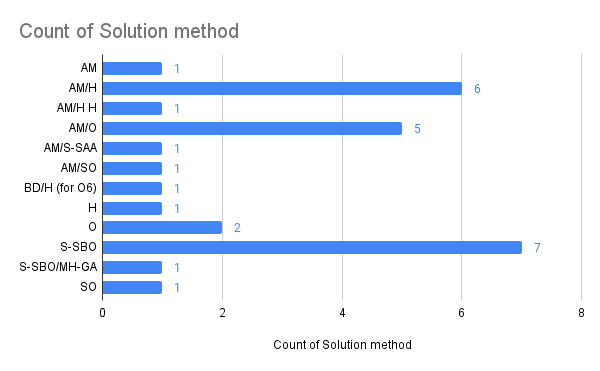
\includegraphics{images/ahmadi1-01.png}

Most solution methods for 1-SSP modeling approaches are analytical or
simulation based (15 and 8 articles, resp.)

\citep{ala_appointment_2022} mention four categories of OASs purposes:

\begin{enumerate}
\def\labelenumi{\arabic{enumi}.}
\item
  Reducing costs
\item
  Increasing patient satisfaction
\item
  Lowering waiting time
\item
  Improving fairness
\end{enumerate}

This will be reflected in the cost function where we will be attempting
to minimize patient waiting times and physician over-time. Fairness is a
rather subjective matter. The cost function will contain weights that
can be adjusted to fit particular cases and/or preferences.

\hypertarget{problem-description-and-solution-methods}{%
\section{Problem description and solution
methods}\label{problem-description-and-solution-methods}}

A schedule is a vector \(x\) consisting of \(T\) elements in which each
element represents the number of patients scheduled at the interval
starting at \(t\):

\[
x = [x_0, x_1, ....x_{T-1}]
\]

with

\[
\displaystyle\sum_{t=0} ^{T-1} x_t = N,\ x_t \in \mathbb{N}_0
\]

Patients are scheduled at fixed intervals with length \(d\).

\begin{figure}

{\centering 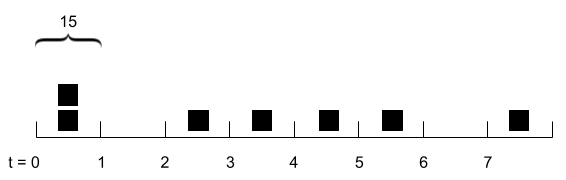
\includegraphics{images/schedule.png}

}

\caption{A schedule
\(x = [2, 0, 1, 1, 1, 1, 0, 1],\ T = 8,\ N = 7,\ d = 15\)}

\end{figure}

Each patient has two endogenous features: type and service time, which
are both independent and identically distributed variables. In our model
we assume there are two patient types: standard and emergency. There is
a probability \(q\) that a patient has an emergency. Service times have
known distributions with mean \(\beta_s\) and \(\beta_e\) for standard
and emergency patients respectively.

All standard patients are assumed to be punctual. The arrival rate of
emergency patients has a Poisson distribution with rate \(\lambda\) per
interval. Emergency patients get priority over standard patients that
are waiting. If several emergency patients are waiting they are served
in order of arrival.

The cost function consists of three elements:

\begin{enumerate}
\def\labelenumi{\arabic{enumi}.}
\tightlist
\item
  The waiting time for patients: \(W(x)\)
\item
  The lateness or over-time of physicians: \(L(x)\)
\item
  The waiting or idle time for physicians: \(I(x)\)
\end{enumerate}

and becomes:

\[
C(x) = \alpha W(x) + \beta L(x) + \gamma I(x)
\]

The weights \(\alpha, \beta,\gamma \geq0\) can be set to reflect the
relative importance of each cost element.

The goal is to find a schedule \(x\) that minimizes the cost function
\(C(x)\):

\[
min\{C(x)|\displaystyle\sum_{t=0} ^{T-1} x_t = N, x_t \in \mathbb{N}_0\}
\]

\textless\textless Description solution method
here\textgreater\textgreater{}

\hypertarget{results}{%
\section{Results}\label{results}}

\hypertarget{discussion}{%
\section{Discussion}\label{discussion}}

\hypertarget{conclusion}{%
\section{Conclusion}\label{conclusion}}

\hypertarget{supporting-information}{%
\section{Supporting information}\label{supporting-information}}

\hypertarget{acknowledgments}{%
\section{Acknowledgments}\label{acknowledgments}}


\nolinenumbers
\renewcommand\refname{References}
  \bibliography{bibliography.bib}

\end{document}
